\long\def\maketitleframe{
\begin{frame}{\alert{Aufnahme} der Hybrid-Vorlesung}{\alert{Achtung Aufnahme!}}
\tikz[overlay, remember picture, opacity=0.4]
\node[xshift=9cm,yshift=1cm, anchor=north west]{
  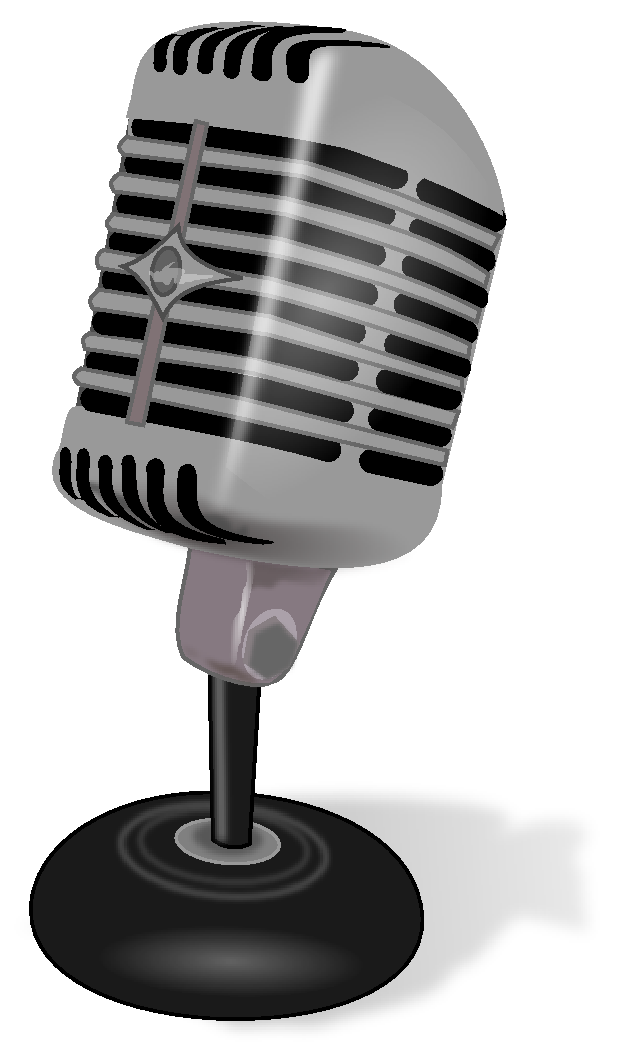
\includegraphics[width=2cm]{fig/microphone-antigo.pdf}
};

\btUseExtraItemSep
\bi
    \ii \textbf{Hybrid-Vorlesung mit Aufnahme}{
      \bi
      \ii Die Aufnahme ist anschließend in Stud.IP verfügbar
      \ii Nutzen Sie die Gelegenheit zur Live-Veranstaltung!
      \ei
    }
    \ii Wir nehmen auf {
      \bi 
      \ii Folien, Dozent, Live-Audio sowie BBB-Audio
      \ii \alert{Ihre Stimme} beim Fragen und Sprechen
      \ii \textbf{Durch aktive Teilnahme erklären Sie sich einverstanden!} 
      \ei
    }
    \ii Fragen: Live, im Chat, Sprechen in der BBB-Sitzung
\ei
\end{frame}

  \begin{frame}[title]
    \maketitle
  \end{frame}
}



\newcommand{\dividerframe}[1]{
  \begin{frame}
    \begin{center}
      \Huge #1
    \end{center}
  \end{frame}
}
